\chapter{Introduction}

\section{Motivation}
The investigation and manipulation of quantum systems are crucial for various applications and technological advancements, as well as for addressing fundamental research questions in physics. In recent years experiments progressed rapidly and we are seeing new technologies emerge in quantum science \cite{QS_1,QS_2} such as quantum computers \cite{quantumcomp1, quantumcomp2}, quantum simulators \cite{quantumsimulators1} and much more.\\

Here quantum optics is such a branch of quantum systems which explores the fundamental interactions between light and matter at the quantum level. It delves into phenomena such as photon entanglement, quantum coherence, and the manipulation of quantum states of light. The study of quantum optics has led to groundbreaking advancements in quantum computing, secure communication \cite{quantuminformation}, and precision measurement technologies \cite{Heeg2017}.\\

Central to quantum optics is the understanding of how light interacts with atomic and molecular systems. These interactions are characterized by phenomena such as spontaneous and stimulated emission, absorption, and scattering, all of which are governed by the principles of quantum mechanics. Relatively new, the field has expanded to encompass X-ray quantum optics, where similar principles are applied to much shorter wavelengths \cite{scientific_opp_XFEL}. X-ray photons, with their higher energies, provide unique opportunities to probe matter with atomic-scale resolution and to explore new regimes of light-matter interaction. X-ray quantum optics opens up possibilities for investigating phenomena such as quantum control of excitons \cite{Heeg2021}, and the development of novel spectroscopic techniques.\\

One of the most intriguing intersections of quantum optics and X-ray physics is found in the study of the Mössbauer effect. The Mössbauer effect, discovered by Rudolf Mössbauer in 1958 \cite{Mssbauer1958}, involves the recoil-free emission and absorption of gamma rays by atomic nuclei bound in a solid. Due to the narrow linewidth of Mössbauer nuclei, this effect provides a highly precise method for examining hyperfine interactions and allows for the study of extremely narrow spectral lines, which are invaluable in various scientific applications such as in materials science, chemistry, and biology. Other than the x-ray quantum optics, Mössbauer effect finds its way in other very diverse areas, such as archaeology \cite{Wagner2004_archeology}, battery development \cite{Lippens2021_battery} and more recently, planetary exploration with a Mössbauer spectrometer sent to Mars on the Mars Exploration Rover to search for water \cite{Klingelhofer2004_mars}.\\

Moreover, in nuclear quantum optics \cite{Adams2013}, many optical schemes have been successfully adapted to the x-ray regime, including Lamb shift \cite{collectivelambshift}, superradiance \cite{superradiance}, electromagnetically induced transparency \cite{EITinxray}, spontaneously generated coherences \cite{spontaneouslygeneratedcoherences}, among others. \\

The main limiting factor in nuclear quantum optics is the current light sources, such as PETRA \MakeUppercase{\romannumeral 3} at DESY in Hamburg \cite{desy} or ESRF in Grenoble \cite{esrf}, which can deliver on average less than one resonant photon per pulse due to the narrow linewidth. As a result, experiments on Mössbauer nuclei have been restricted to low-excitation regime (LER) so far. Attempts to achieve higher excitations and nuclear inversion was a long standing dream \cite{oldproblem1,oldproblem2,oldproblem3}.   \\

However, with self seeded x-ray free electron lasers (XFEL) \cite{xrayFEL, XFEL2} in the hard x-ray regime, a significant improvement of the number of nuclear-resonant photons per pulse on average \cite{Shvydko2023,superradiance} can be achieved. Additionally, by utilizing advanced measuring schemes and improved focusing techniques \cite{dominik_higherexcitation}, achieving higher excitations beyond the low-excitation regime is becoming increasingly feasible.\\

Theoretically, the interaction between light and matter is described by the Maxwell-Bloch equations. In general, it is not possible to solve the Maxwell-Bloch equations analytically. Nevertheless under certain conditions analytical results can be obtained. For example, in the low-excitation regime these equation can be solved to obtain the \textit{response function}, a well-established technique to describe the nuclear dynamics \cite{Rhlsberger2005}. This attempt can be expended with a perturbation approach as in \cite{wolff2023characterization}. In this work they derived a ratio between the coherent and incoherent light that remains constant over time within the LER but varies beyond it, which then can be used to evaluate the regime that one operates the experiment. This is an important tool to differentiate the different levels of excitations, especially in the time where due to the x-ray free electron lasers more and more resonant photons per pulse can be generated. The main results of this work are shown in \Cref{fig:lukas_result}. However, they did not take into account the effects resulting from propagation of light through thick targets. \\

Another possibility to solve the Maxwell-Bloch equations analytically is to consider the times much shorter compared to the characteristic decay of the excited states \cite{BURNHAM1969}. Burnham et.al. developed a model that approximates the light propagation and nuclear dynamics in an excitation regime from the LER to population inversion. \\
\begin{figure}
    \centering
    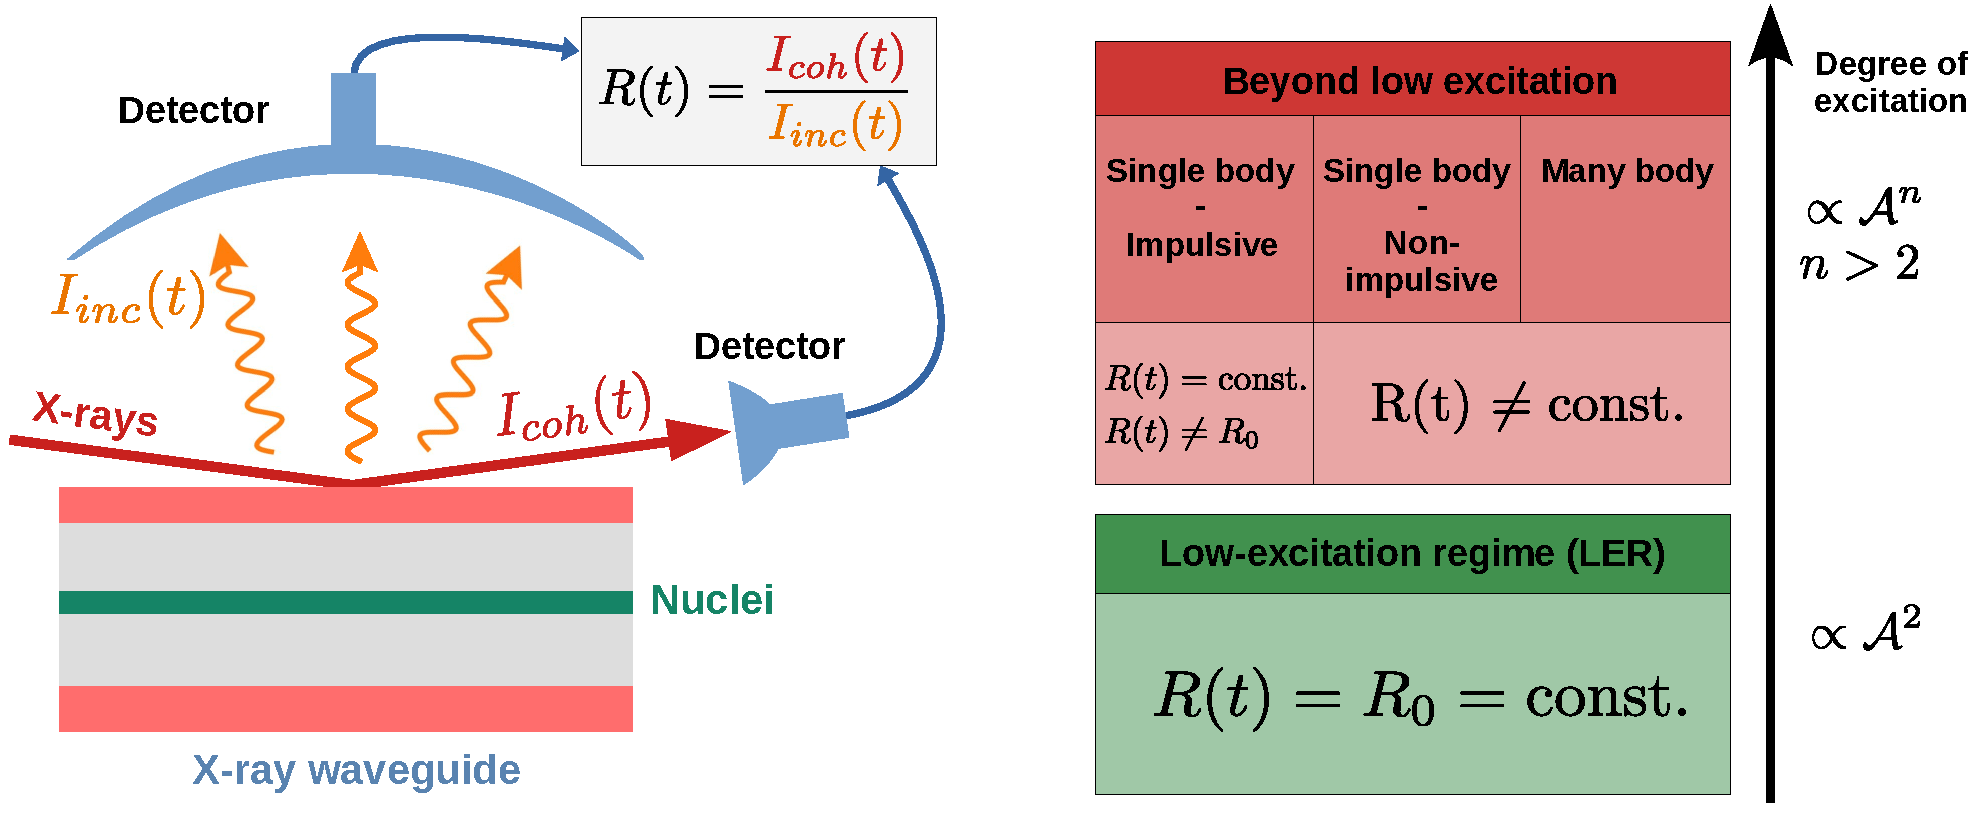
\includegraphics[width =0.75\textwidth]{data/introduction/OverviewPicture.pdf}
    \caption{Characterization and detection method for x-ray excitation beyond the low-excitation regime. Here the main results are displayed from \cite{wolff2023characterization}. In this work, they were able to show that the ratio of coherent to incoherent light stays constant over time in the low excitation regime. For coherent light $I_\mathrm{coh} = |\rho_{eg}|^2$ and for incoherent light $I_\mathrm{inc} = \rho_{ee}$ was used, as there were no propagation effects taken into account. (This figure is reproduced with the permission of the authors \cite{wolff2023characterization}.)} 
    \label{fig:lukas_result}
\end{figure}


\section{Goals of this thesis}

In this thesis, we want to extend the previous works in two directions which can be seen in \cref{fig:model_comp}. First, we want to analyse stronger excitations even beyond inversion and secondly we want to include propagation effects in thicker targets. Our objectives include comparing the dynamics within the low excitation regime (LER) under without propagation effects with the results presented in \cite{wolff2023characterization} and extend the analysis to thicker targets, where propagation effects have to be taken into account. Subsequently, we want to investigate dynamics beyond the low excitation regime under the non-decaying limit ($\gamma = 0$) and compare our results with those of \cite{BURNHAM1969}. Additionally, we will explore the decaying limit beyond the low excitation regime and population inversion, uncovering interesting structures. Finally, we will propose an experimental signature capable of detecting nonlinear excitation through the time shifts of intensity minima.\\

\begin{figure}
    \centering
    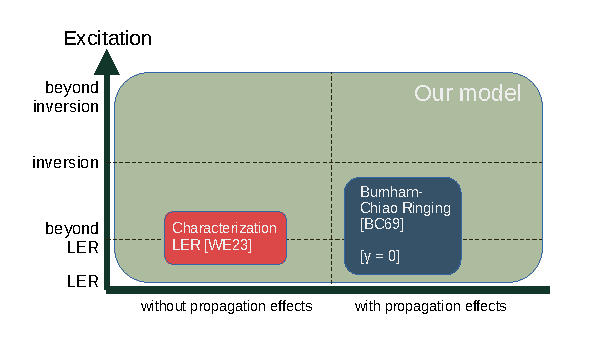
\includegraphics[width = 0.85\textwidth]{data/introduction/resultsvergleich_2.pdf}
    \caption{An overview is given to compare the limits of different models. \cite{wolff2023characterization} proposes methods to characterize the low-excitation regime without taking into account the propagation effects. On the other hand, \cite{BURNHAM1969} gives a model that approximates the dynamics from LER to population inversion in the non-decaying limit. With our model, we can analyse the low excitation regime as well as higher excitations and beyond the population with propagation effects and spontaneous decay.}
    \label{fig:model_comp}
\end{figure}


\section{Thesis outline}

In Chapter 2, an introduction will be provided to quantum optical two-level systems and light-matter interactions. The Maxwell-Bloch equations will be presented, and the response function formalism in the time domain will be derived. Additionally, the results from Burnham and Chiao \cite{BURNHAM1969} will be summarized. In Chapter 3, the method of lines will be introduced. This method will be used to discretize the spatial component of the Maxwell-Bloch equations. Consequently, this discretization will enable us to solve coupled ordinary differential equations instead of a partial differential equation. In Chapter 4, we will present our results. The first half focuses on the Low Excitation Regime (LER), where we compare our findings with those of \cite{wolff2023characterization} and extend them to include the propagation limit. The second half delves into dynamics beyond the LER and population inversion, where we compare our results under the non-decaying limit and generalize to the decaying limit. In Chapter 5, a summary of the findings will be presented, highlighting key insights and conclusions drawn from the study. Additionally, an outlook will be provided, discussing the applicability of the developed model in other settings.
